\pdfmapfile{+univers}%
\pdfmapfile{+dinbold}%
\documentclass[ngerman]{beamer}
\usepackage[utf8]{inputenc}
\usepackage[T1]{fontenc}
\usepackage[ngerman]{babel}
\usepackage{graphicx}
\usepackage{svg}
\usetheme[pagenumbers=full,transition=push,headline=light]{tud}
\begin{document}
\title{FoodShip}
\subtitle{FoodShip, a foodsharing App}
\author{Sönke Huster \& Hannes Hilbert}
\date{\today}

\maketitle

%\frame{\frametitle{Inhaltsverzeichnis}\tableofcontents}

\section{Vorstellung}
\subsection{App Idea}
\frame{\frametitle{App Idea}
Hier die App Idee
}

\subsection{Mockups}
\frame{\frametitle{Mockups}
\begin{figure}
  \centering
  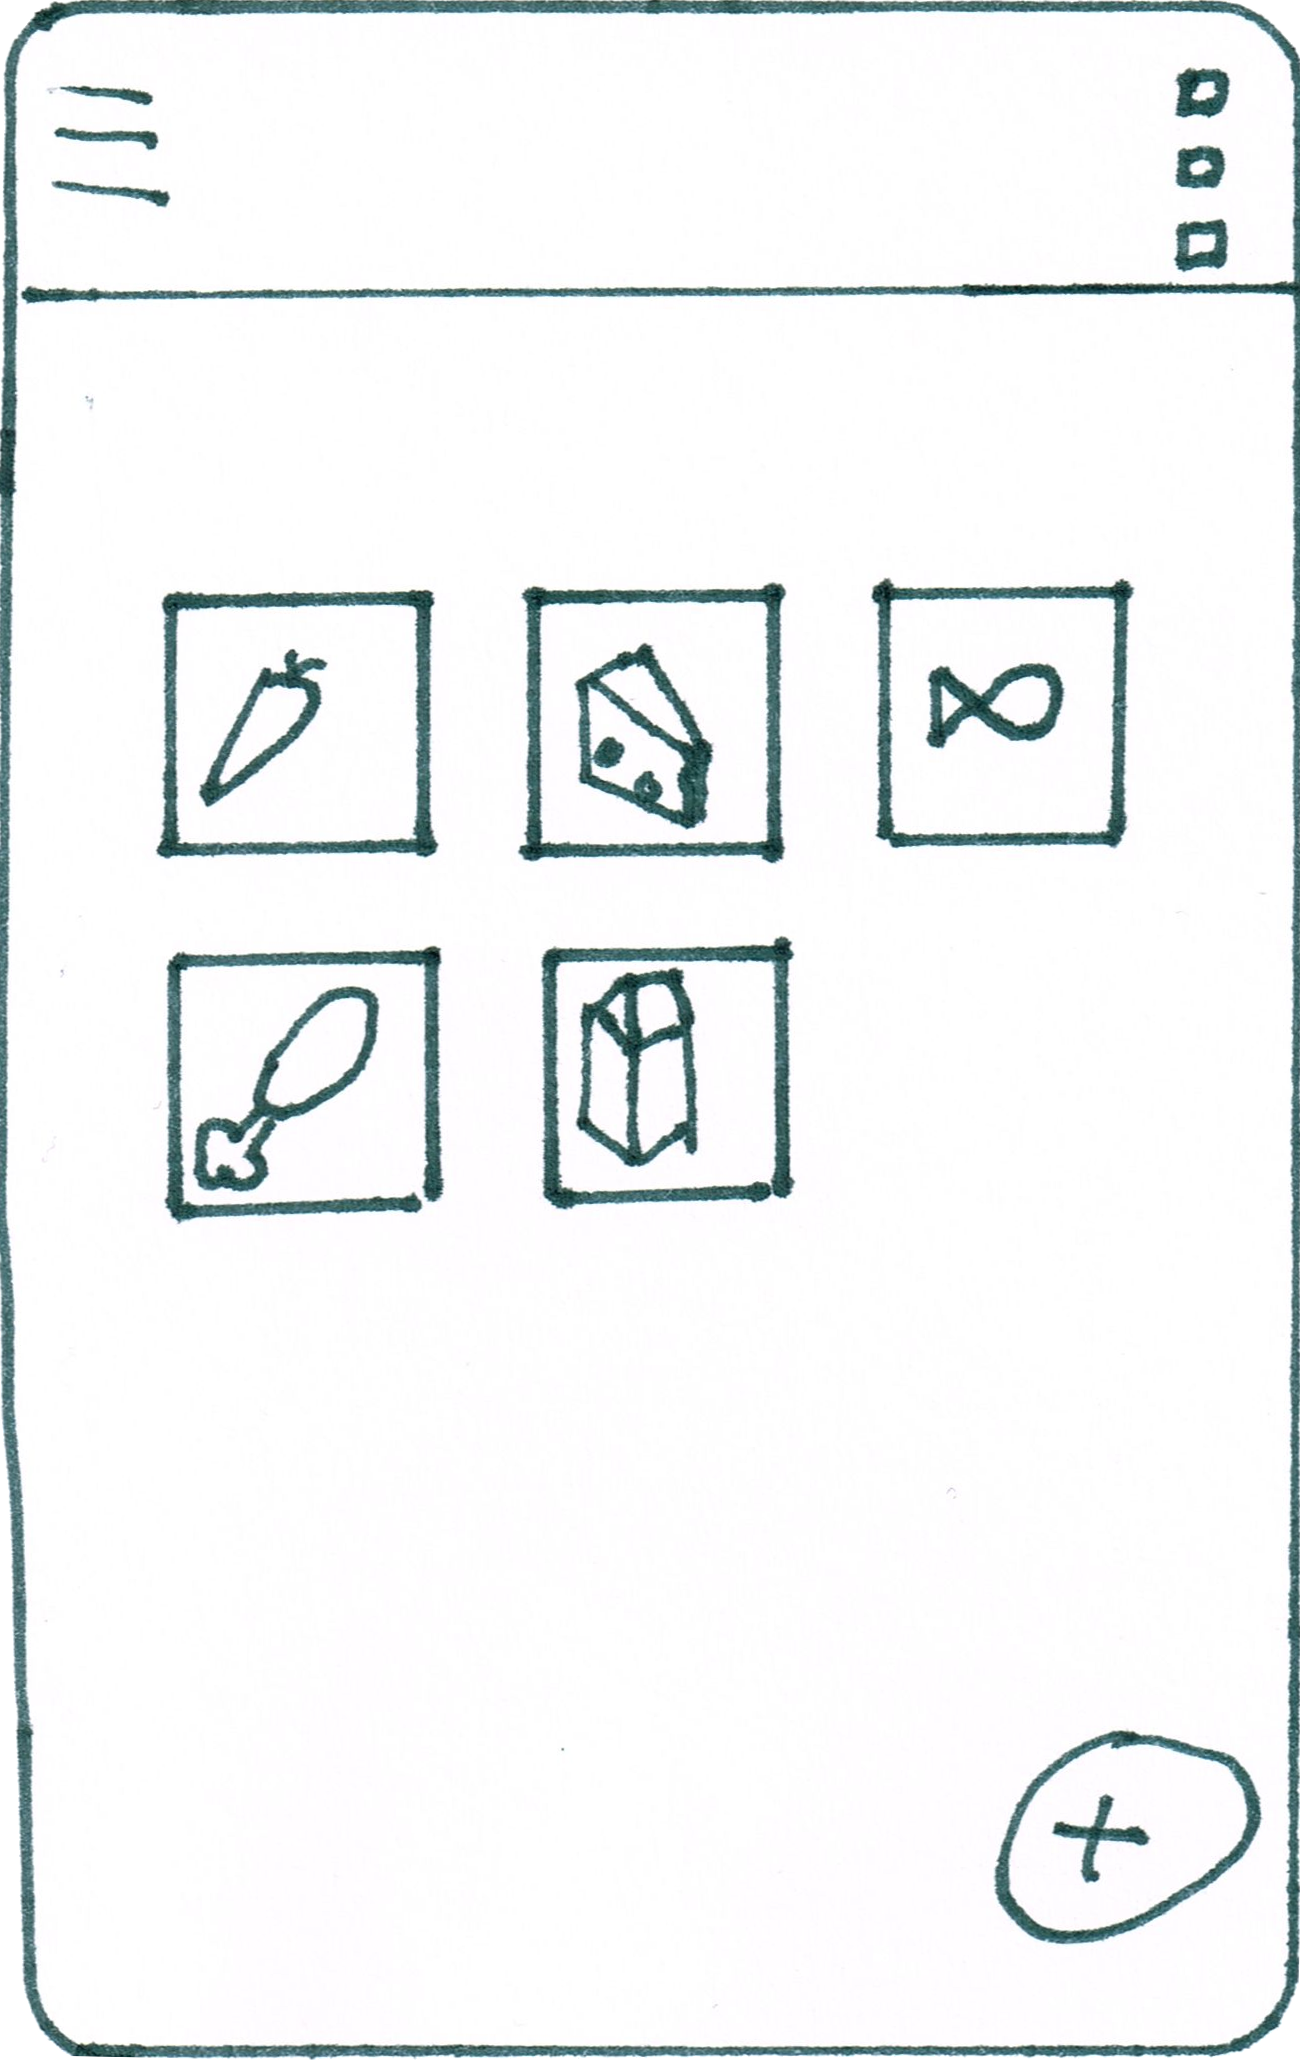
\includegraphics[width=0.4\textwidth,height=0.8\textheight,keepaspectratio]{../mockups/food-home-overview.png}
   \vspace{10cm}
  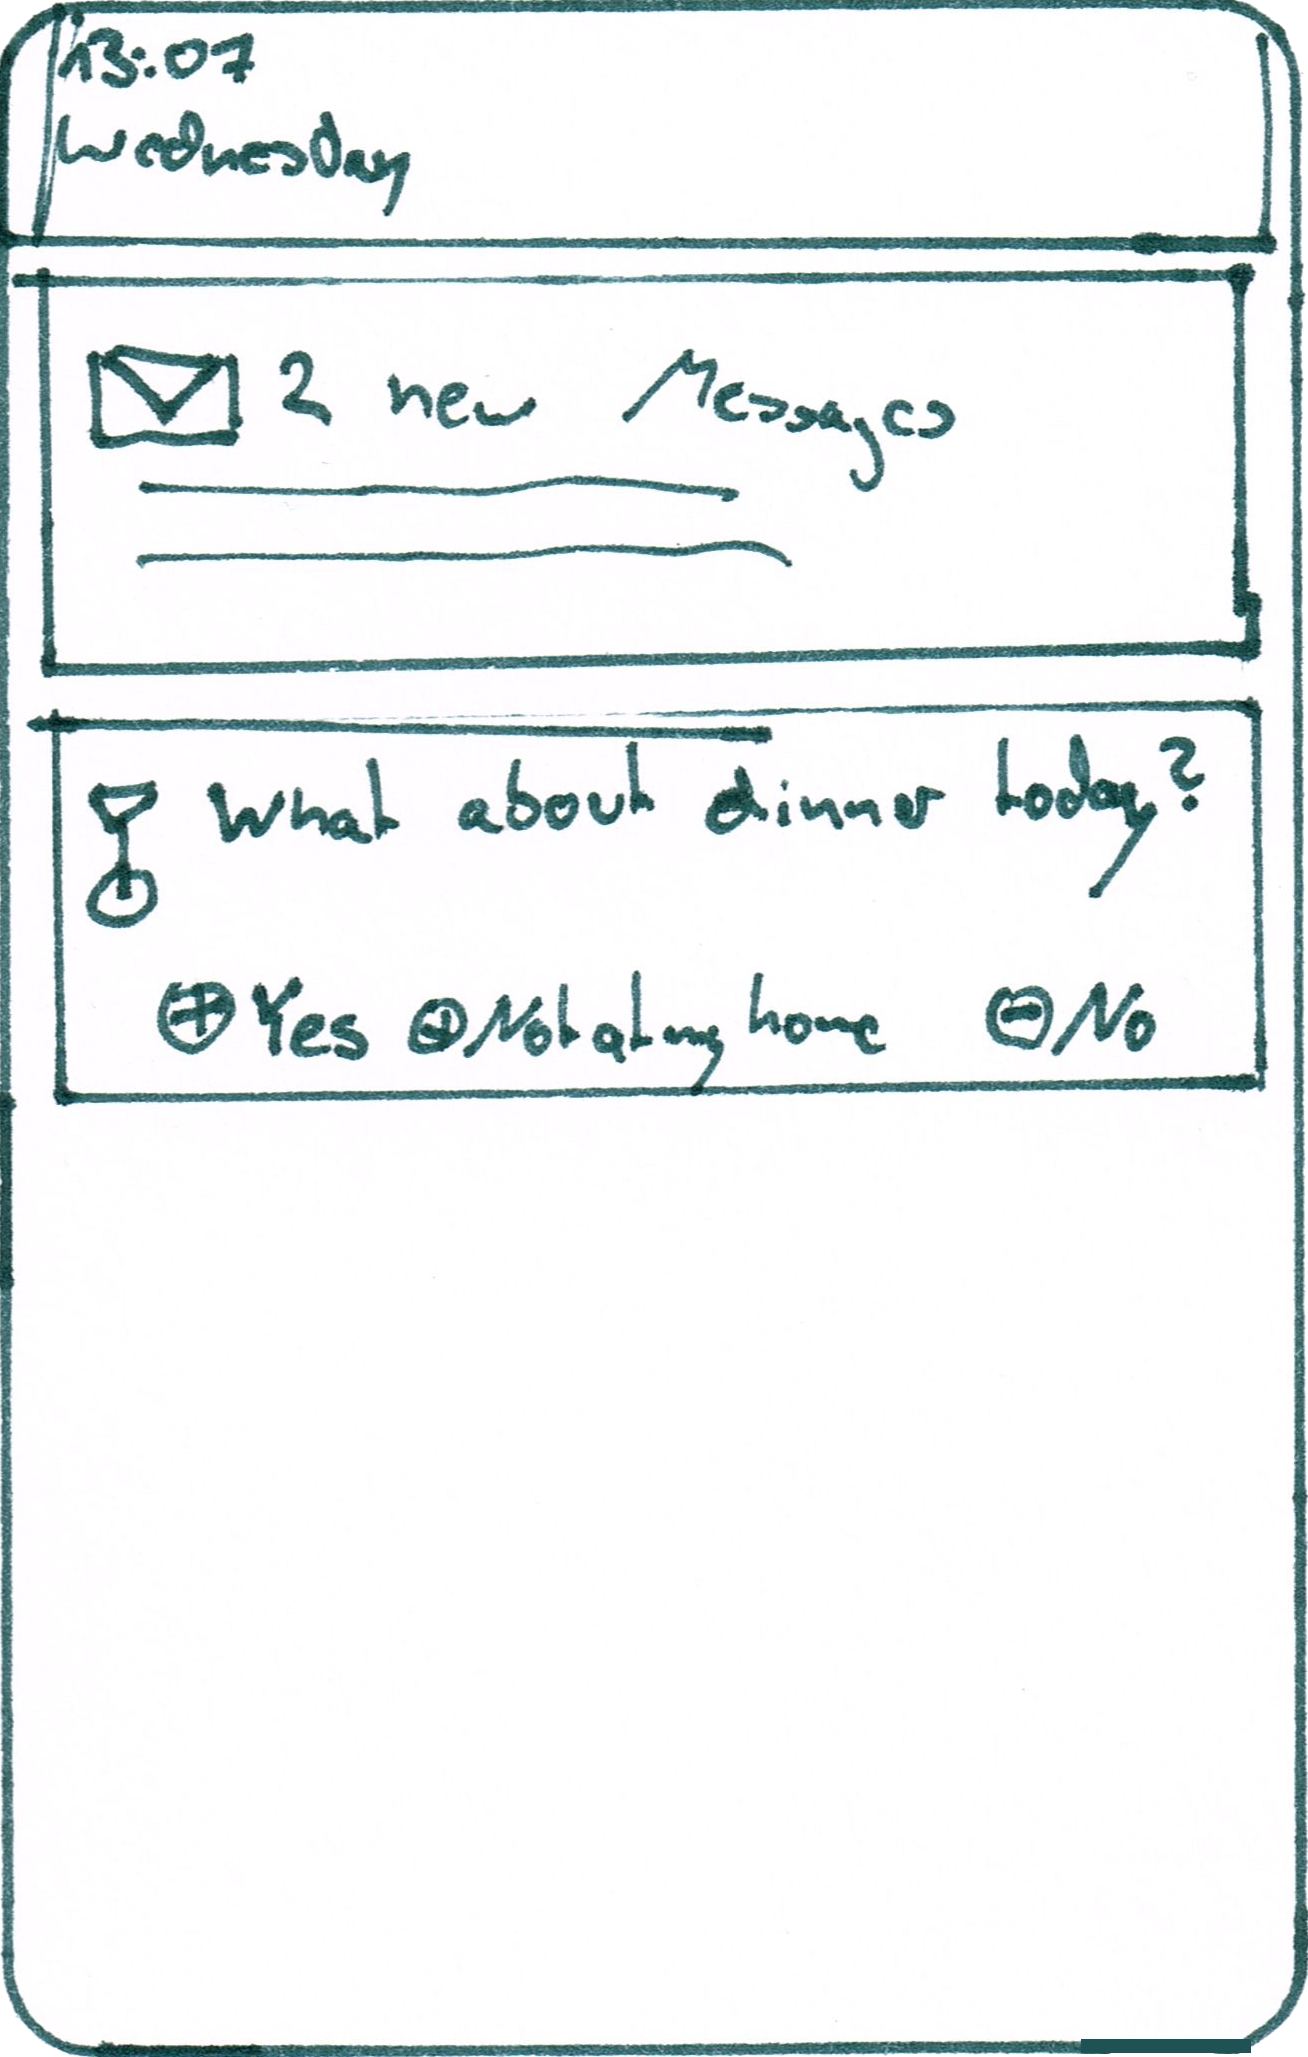
\includegraphics[width=0.4\textwidth,height=0.8\textheight,keepaspectratio]{../mockups/notification.png}

\end{figure}
}

\frame{
\begin{figure}
  \centering
  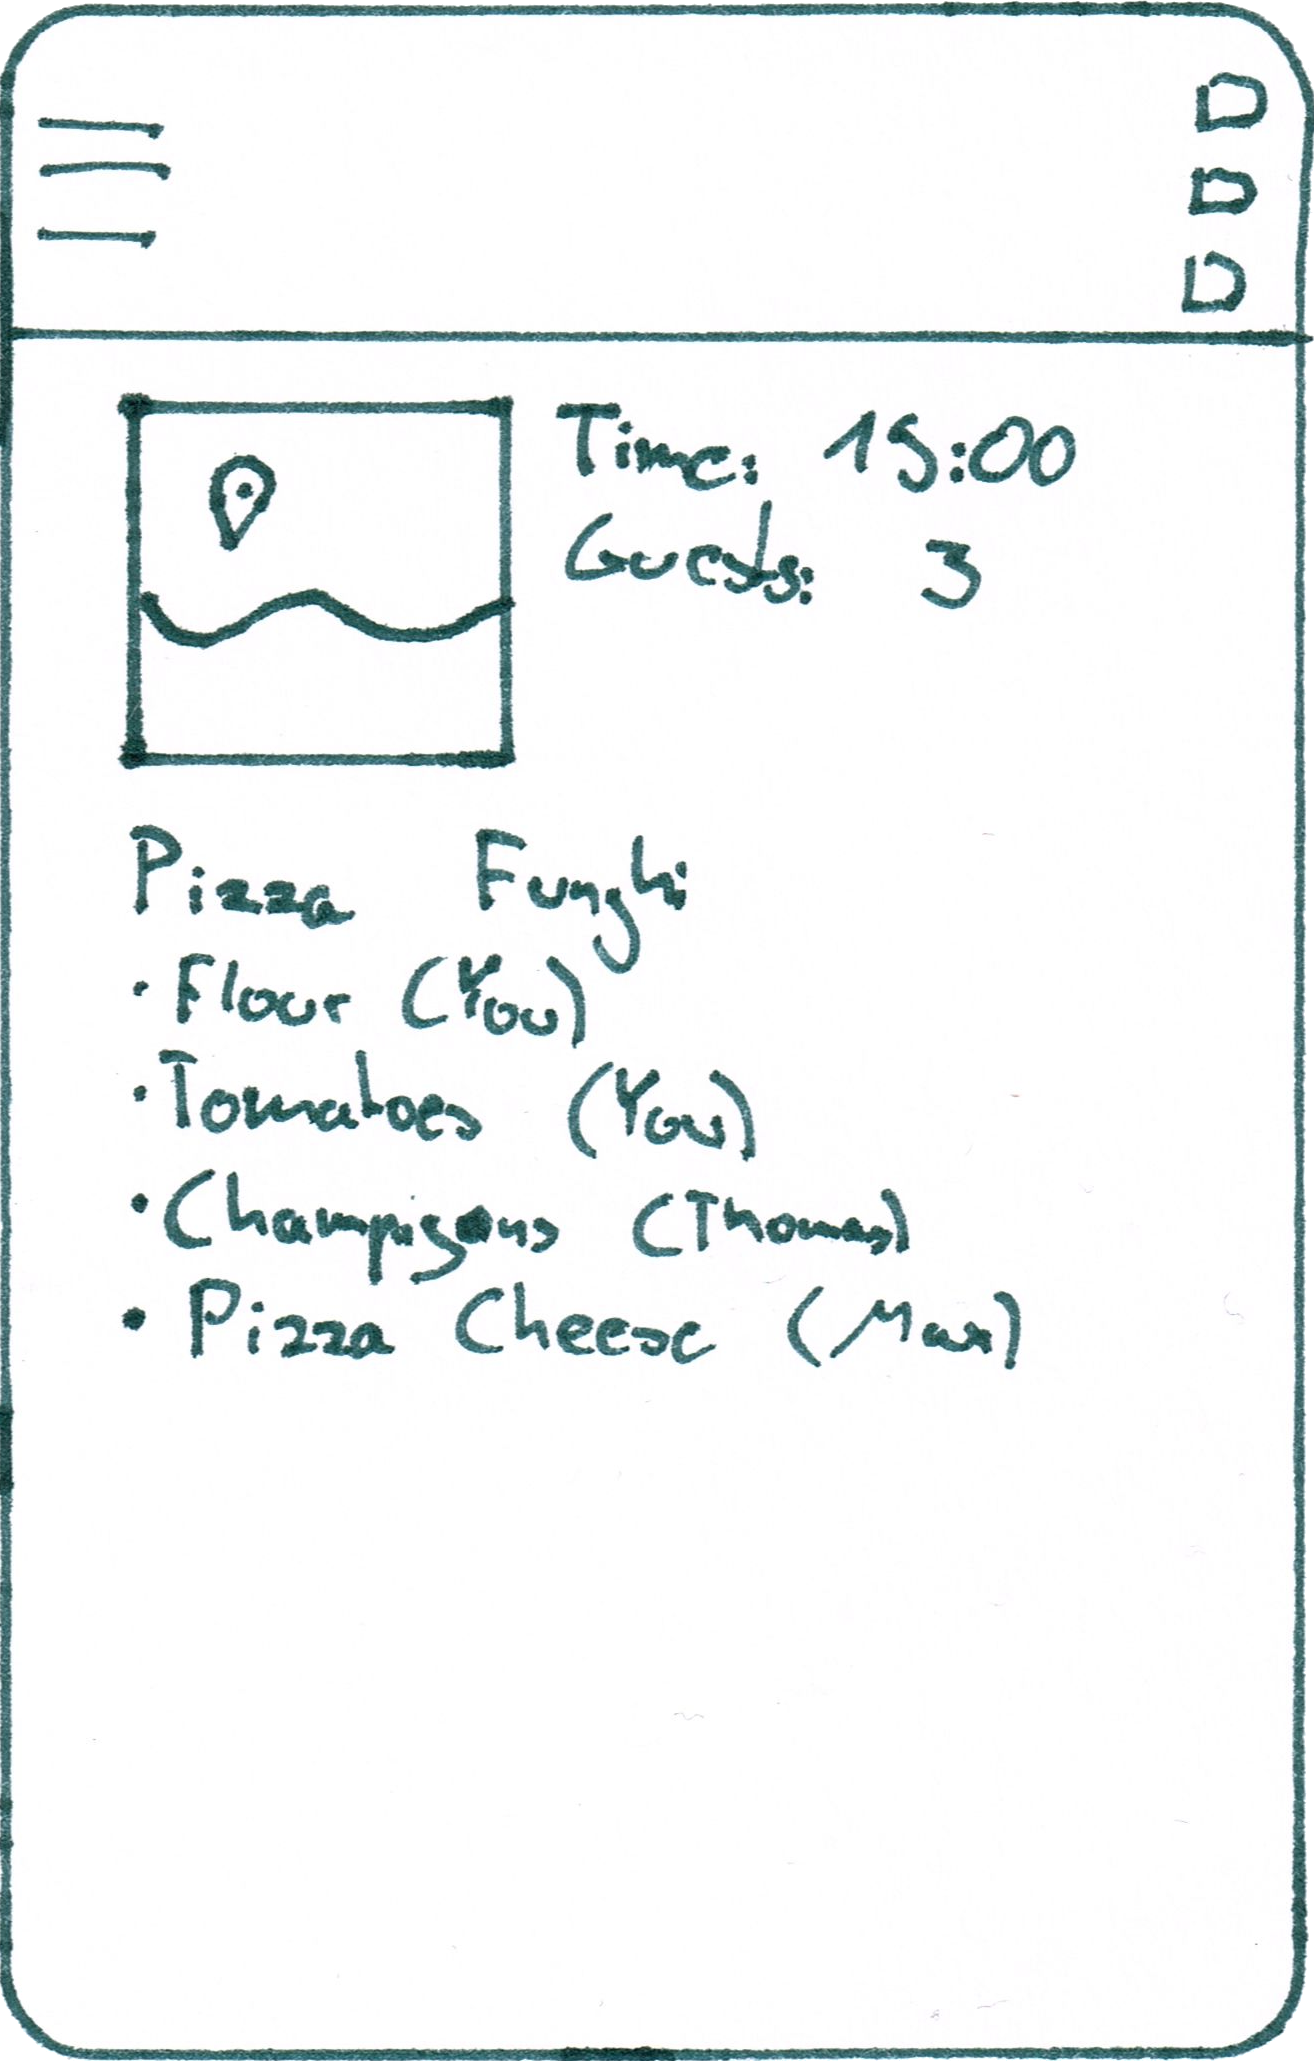
\includegraphics[width=0.4\textwidth,height=0.8\textheight,keepaspectratio]{../mockups/dinner-overview.png}
   \vspace{10cm}
  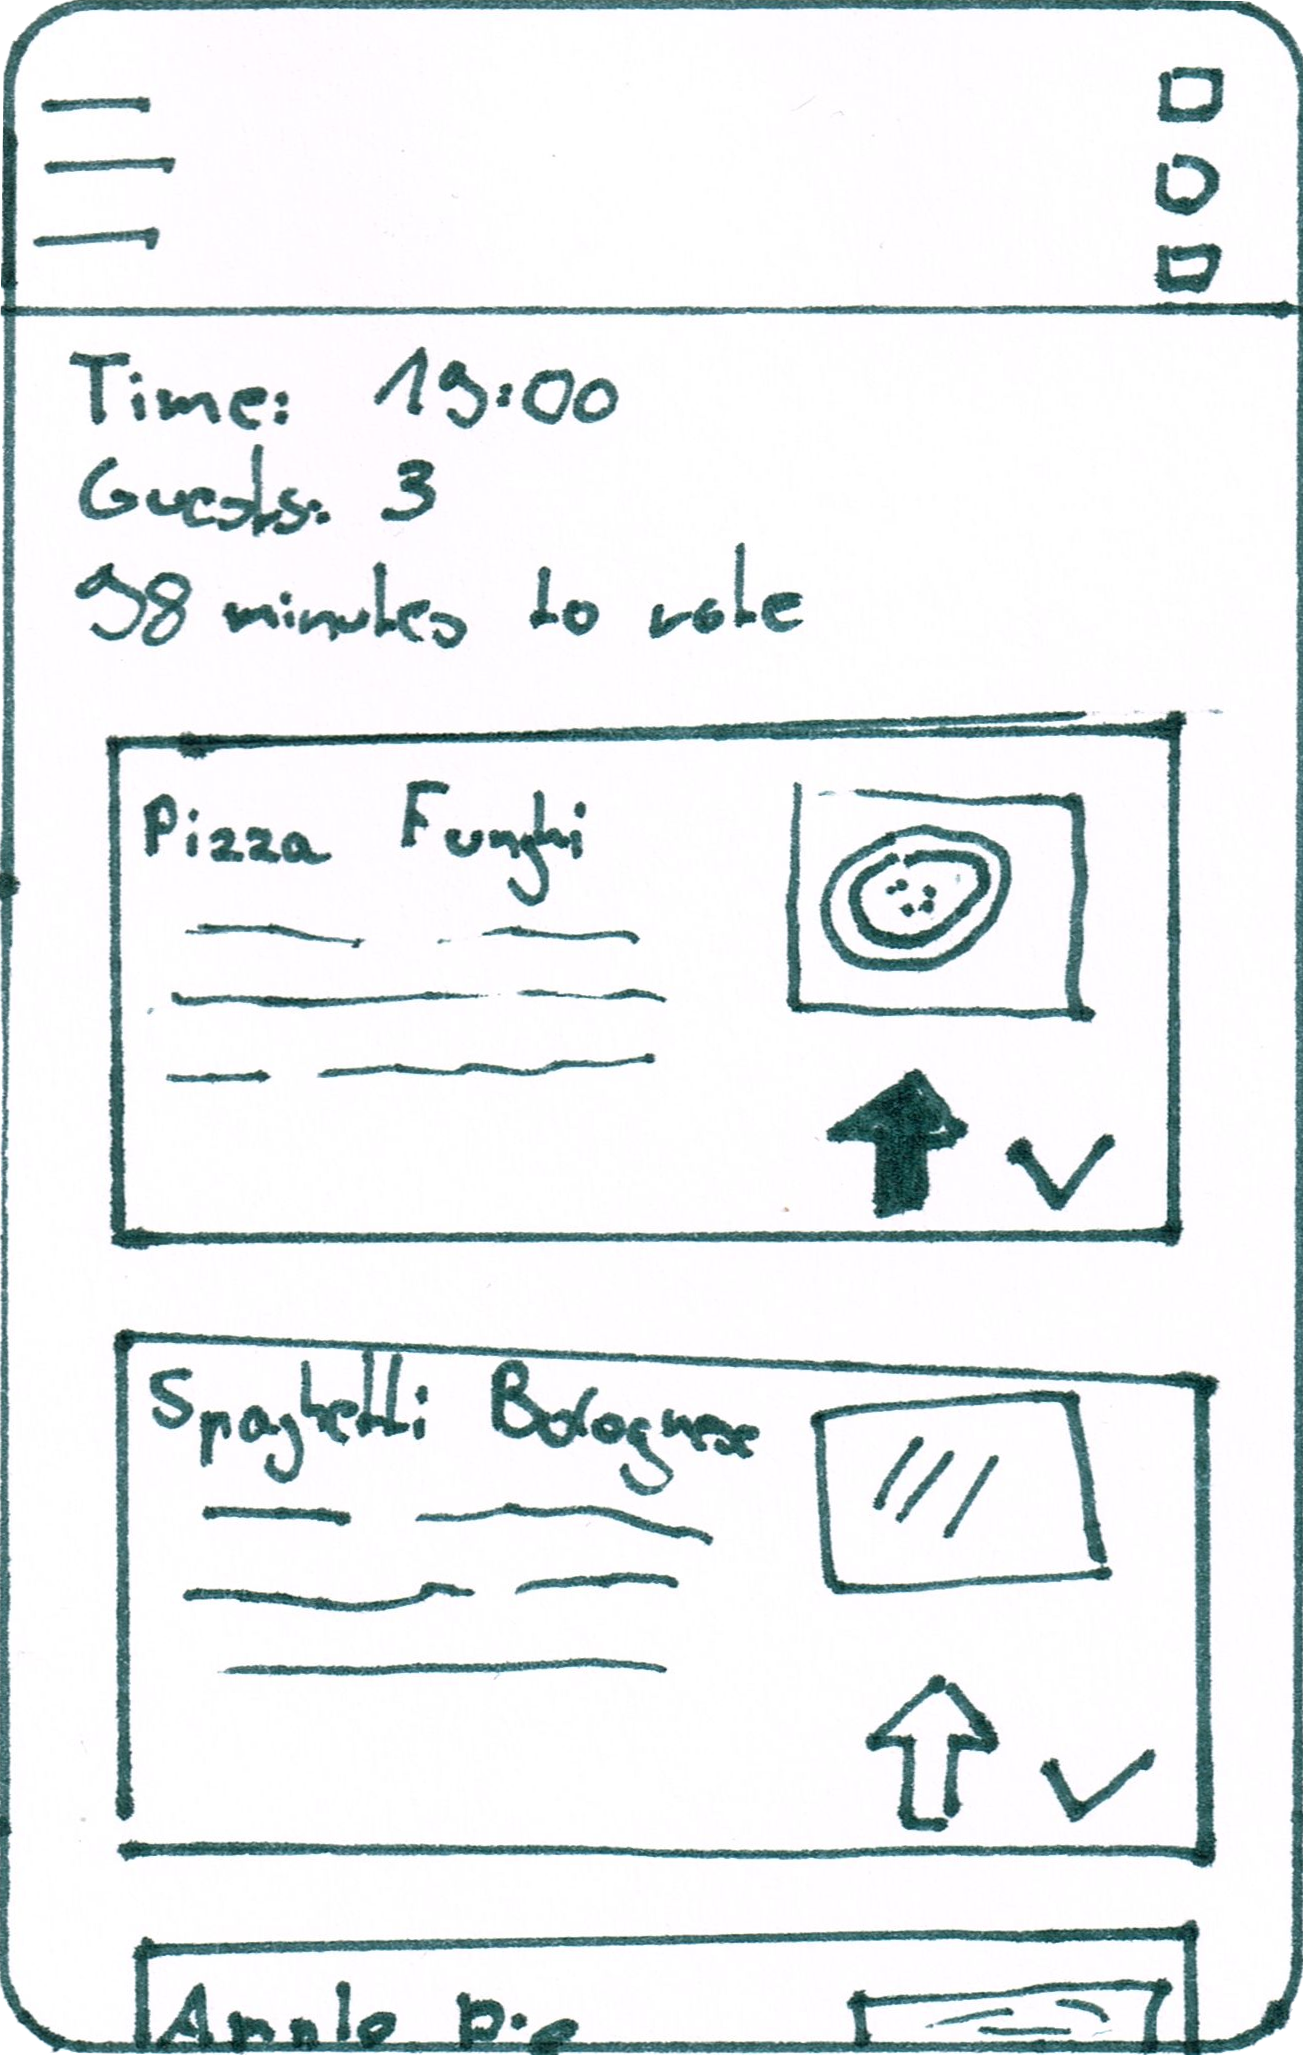
\includegraphics[width=0.4\textwidth,height=0.8\textheight,keepaspectratio]{../mockups/dinner-recipe-voting.png}
\end{figure}
}


\subsection{Use Cases}
\frame{\frametitle{Use Cases}
}

\section{Callenges}
\frame{\frametitle{Callenges}

\begin{itemize}
\item  Callenge 1
\item  Callenge 2
\item  Callenge 3
\end{itemize}
}
\section{App Development}
\subsection{Technologies}
\frame{\frametitle{Technologies}
\begin{itemize}
\item  Andriod:
\begin{itemize}
  \item{Bla}
\end{itemize}
\item  Server:
\end{itemize}
}

\subsection{Architecture}
\frame{\frametitle{Architecture}
\begin{figure}
  \centering
  \includegraphics[width=0.9\textwidt,height=\textheight,keepaspectratio]{../diagrams/architecture.png}
\end{figure}
}

\subsection{Workplan}
\frame{\frametitle{Workplan}
\begin{itemize}
  \item Los
\end{itemize}}
\end{document}
